\section{Formeln}

\textit{Basiseinheiten: Meter m, Kilogramm kg, Sekunde s, Ampere A, Kelvin $\vartheta$, Mol mol, Candela cd} \\
\begin{minipage}{12cm}
	Kraft: $\overrightarrow{F} = m \cdot a$ \\ 
	Ladung: $Q = I \cdot t$\\
%	Spannung: $U = W \cdot Q = R \cdot I = E \cdot l_{AB} = \varphi \textsubscript{A} - \varphi \textsubscript{B}$\\
	$ U_{AB} = \varphi_A - \varphi_B $ = $\int\limits_{A}^B \vec E (s) \cdot  \vec{ds} \overrightarrow{}$ im homogenen Feld: $U_{AB} = E \cdot \overline{AB} \cdot \cos\alpha $ \\
	Strom: $I = \frac{\Delta Q}{\Delta t} = \frac{U}{R} = J \cdot A = \frac{U \cdot \sigma \cdot A}{d} = \int\limits_{A} \vec J \cdot d\vec A = J \cdot A = J \cdot A \cdot cos \varphi $\\
	Stromdichte: $J=\frac {I}{A} = \frac{U \cdot \rho}{d} = \sigma \cdot \vec E $\\
	Arbeit: $W = F \cdot s$ \\
	Energie"anderung: $\Delta W = \Delta Q \cdot U = e \cdot U_{AK} = \frac{1}{2} \cdot m_{e}  \cdot v^2 = \\ P \cdot \Delta t = U \cdot I \cdot \Delta t$ \\
	Leistung = $P = \frac{\Delta W}{\Delta t}= U \cdot I = \frac{\Delta Q \cdot U}{\Delta t} = I^2 \cdot R = \frac{U^2}{R} $\hspace{10pt}\\
	Leistungsdichte $\frac{\Delta P}{\Delta V} = \frac{\Delta U }{\Delta l} \cdot \frac{\Delta I}{\Delta A} = E \cdot J = \sigma E^2 = \rho \cdot J^2 $\\
	Linearer Widerstand: $R = \frac{U}{I} = \frac{\rho \cdot d}{A} = \frac{d}{\sigma \cdot A} \; $\\
	Nicht linearer Widerstand: $R(I) = \frac{\Delta U}{\Delta 1}$ \\
	Spezifischer Widerstand: $R = \frac{\rho\mathit{l}}{A}=\frac{\mathit{l}}{\sigma \cdot A}$\\
	Leitwert: $G = \frac{1}{R}$ \\
	Materialabhängiger spezifischer Widerstandswert: $\rho_{20} = \frac{R \cdot A}{l} $\\
	Temperaturkoeffizient bzgl 20$^\circ$: $\alpha_{20}=\frac{\Delta R}{ R_{20} \cdot \Delta \vartheta}$ \\
	Leitf"ahigkeit: $\sigma = \frac{1}{\rho}$ \\
	Elektrisches Feld: $\overrightarrow{E} = \frac{\overrightarrow{F}}{Q} = \frac{U}{d} = \frac{J}{\sigma} = \rho \cdot \vec J $\\
	W"armemenge: $Q = m \cdot c_{p} \cdot \Delta\vartheta$ \\
	Kapazit"at: $C = \frac{Q}{U}$

\end{minipage}
\begin{minipage}{5cm}
	$\left[F\right] = \frac{1kg \cdot m}{s^2} = 1N$ \\
	$\left[Q\right] = 1 As = 1 C$ \\
	$\left[U\right] = \frac{\lbrack W \rbrack}{\lbrack Q \rbrack} =\frac{1 J}{C} = \frac{1kg \cdot m^2}{A \cdot s^3} = 1 V$ \\
	$\left[I\right] = A $ \\
	$\left[J\right] = \frac {A}{m^2} $\\
	$\left[W\right] = \frac{1kg \cdot m^2}{s^2} = 1Nm = 1 J \; (Joul) = 1 Ws$ \\
	$ \left[P\right] = V \cdot A = W (Watt)$\\
	$\left[G\right] = \frac{A}{V} = S \, (Siemens) = \frac{1}{\Omega}$\\
	$\left[ \rho \right] = \frac{\Omega \cdot m^2}{m} = \Omega m$  häufig:  $\frac{\Omega \cdot mm^2}{m} $\\
	$\left[ \sigma \right] = \kappa = \frac{1}{\Omega m} = \frac{S}{m} = \frac{m}{\Omega \cdot mm^2} $\\
	$\lbrack \alpha \rbrack = \frac{1}{K}$\\
	$\lbrack C \rbrack = \frac{As}{V} = F \; (Farad)$ \\ 
	$\lbrack E \rbrack = \frac{V}{m} = \frac{N}{C} \; $ (Volt pro Meter) \\ 
\end{minipage}

\begin{minipage}{2.7cm}
	$10^{12} \: T \:Tera$ \\
	$10^9 \: G \: Giga$ \\
	$10^6 \: M \: Mega$ \\
	$10^3 \: k \: Kilo$ \\
\end{minipage}
\begin{minipage}{2.7cm}
	$10^{-12} \: p \:Pico$ \\
	$10^{-9} \: n \: Nano$ \\
	$10^{-6} \: \mu \: Mikro$ \\ 
	$10^{-3} \: m \: Milli$ \\
\end{minipage}
\begin{minipage}{4.5cm}
	$e = 1,062 \cdot 10^{-19} \; C$ \\
	$1\cdot C = 6.241\cdot 10^{18} \; Elektr.$ \\
	$c \approx 300000 km/s$ \\
\end{minipage}
\begin{minipage}{4cm}
	$\sin \beta = \frac ba =\frac{\text{Gegenkathete}}{\text{Hypotenuse}}$\\
	$\cos \beta = \frac ca =\frac{\text{Ankathete}}{\text{Hypotenuse}}$\\
	$\tan \beta = \frac cb =\frac{\text{Gegenkathete}}{\text{Ankathete}}$\\
	$\cot \beta = \frac cb =\frac{\text{Ankathete}}{\text{Gegenkathete}}$\\
\end{minipage}
\begin{minipage}{4cm}
	$Dichte \; \rho = \frac{m}{V} \\
	Volumen \; V = A \cdot l$ \\
	$A_{Kreis} = \pi \cdot r^2 = \pi \cdot \frac{d^2}{4}$ \\
\end{minipage}
$\Delta R = R_{\vartheta}-R_{20} = R_{20} \cdot \alpha_{20} \cdot \Delta \vartheta$ $\rightarrow$ $R = R_{20} \cdot (1 + \alpha_{20} \cdot \Delta \vartheta)$\\
$\alpha$ = Temperaturkoeffizient, $\alpha_{20}=\frac{\Delta R}{ R_{20} \cdot \Delta \vartheta} \rightarrow \lbrack \frac{1}{K} \rbrack$\\
0°C = 273,15K \\
Bei höheren Temperaturen (ab einigen $100^\circ$): \\
$R_{\vartheta} = R_{20} \cdot\left( 1 + \alpha_{20} \cdot \Delta \vartheta + \beta_{20} \cdot (\Delta \vartheta)^2 + \gamma_{20} \cdot (\Delta \vartheta)^3 + ... + k_{n} \cdot (\Delta \vartheta)^n \right) => Taylor  $

\textbf{Äquivalenz zwischen linearer Strom- und Spannungsquellen-Ersatzschaltungen}
\begin{multicols}{3}
	$ U_q = U_0 \; T \overrightarrow{} N \; I_{q} = \frac{U_{q}}{R_{i}} $\\
	$ R_i = \frac{U_q}{I_K} = \frac{U_0}{I_K} $\\
	$ G_i = \frac{I_K}{U_0}\ \ \ \ \ R_i = \frac{1}{G_i}$\\
	$ I_q = I_K \; N \overrightarrow{} T \; U_q = I_q \cdot R_i $\\
	Umwandlung: Ri ist bei beiden gleich!\\
	Spannungsquelle nach Thévenin\\
	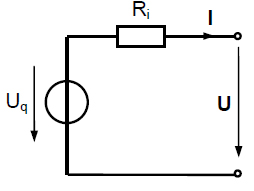
\includegraphics[width=0.13\textwidth]{pics/dcnet/ersatz_spannung}\\
	Stromquelle nach Norton\\
	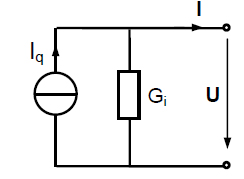
\includegraphics[width=0.13\textwidth]{pics/dcnet/ersatz_strom}\\
\end{multicols}

